\documentclass[twocolumn,superscriptaddress,aps]{revtex4-1}


%%%%%%%%%%%%
% Packages %
%%%%%%%%%%%%

\usepackage[utf8]{inputenc}

\usepackage{amsfonts}
\usepackage{amssymb}
\usepackage{amsmath}
\usepackage{amsthm}

\usepackage{bbold}
\usepackage{bm}
\usepackage{graphicx}
\usepackage{color}
\usepackage{hyperref}


%%%%%%%%%%%%
% Document %
%%%%%%%%%%%%

\begin{document}
    % ----- Title ----- %
    
    \title{\Large{INFO8010 : Neural style transfer}}
    \vspace{1cm}
    
    \author{\small{\bf Maxime Meurisse}}
    \affiliation{\texttt{m.meurisse@student.uliege.be} (\texttt{s161278})}
    
    \author{\small{\bf Adrien Schoffeniels}}
    \affiliation{\texttt{adrien.schoffeniels@student.uliege.be} (\texttt{s162843})}
    
    \author{\small{\bf Valentin Vermeylen}}
    \affiliation{\texttt{valentin.vermeylen@student.uliege.be} (\texttt{s162864})}
    
    \maketitle
    
    %%%%%%%%%%%%%%%%%%%%
    %%%%%%%%%%%%%%%%%%%%
    %%%%%%%%%%%%%%%%%%%%
    
    % ----- Introduction ----- %
    
    % TO DO
    % -----
    % States the problem which has been tackled
    
    \section{Introduction}
    
    We decided to tackle the subject of \emph{neural style transfer} for this deep learning project. The basic idea of this subject is to \emph{merge the style of one image and the content of another image}, for example applying the style of an oil painting to a photo of an animal.\\
    
    An example of such an application is shown in Figure \ref{fig:introduction.example}.\\
    
    \begin{figure}[ht]
        \centering
        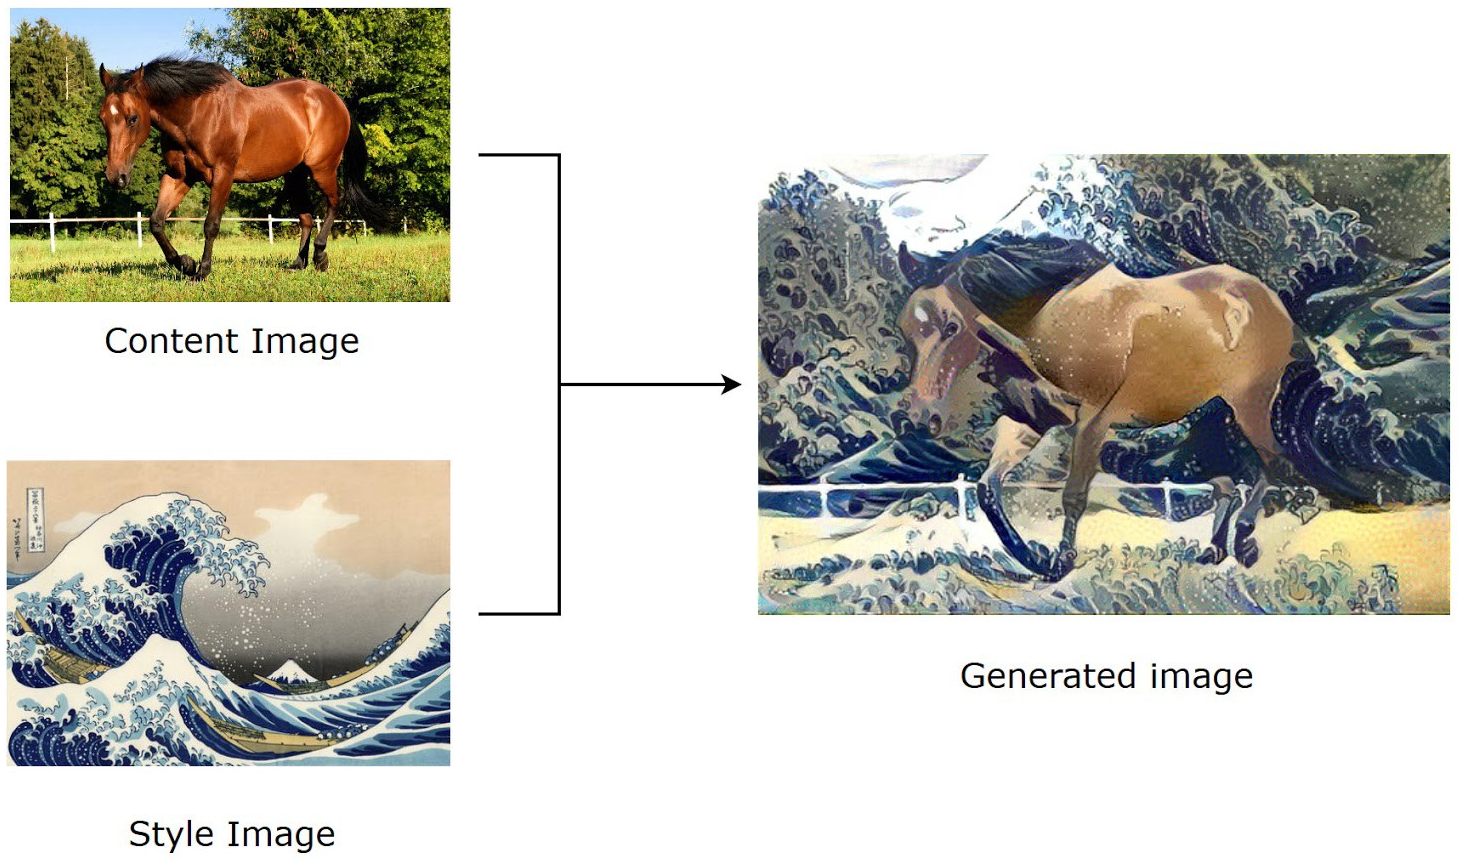
\includegraphics[width=0.45\textwidth]{resources/png/example.png}
        \caption{An example of neural style transfer product \cite{towardsdatascience.com}.}
        \label{fig:introduction.example}
    \end{figure}
    
    However, the rich domain of neural style transfer does not stop there, many other possible applications and extensions exist : modifying the style of a painting to make it look like a photo (and vice versa), modifying the style of certain elements of a photo (for example, transforming horses into zebras by applying a striped texture to them), transforming a summer landscape into a winter landscape, coloring an image, etc.\\
    
    The applications are many and varied. We have chosen to focus on the application of merging the style of an image and the content of another image.\\
    
    To do this, we first started by exploring the technique explained in the paper by Gatys et al. \cite{DBLP:journals/corr/GatysEB15a}. We tried to re-implement this technique ourselves, to improve it, and to vary the different parameters to understand how it works. This method is described in section \ref{methods.gatys} and its results are discussed in section \ref{results.gatys}.\\
    
    Secondly, we have looked at the CycleGAN (\emph{Cycle-Consistent Generative Adversarial Networks}) technique introduced in the paper by Zhu et al. \cite{DBLP:journals/corr/ZhuPIE17}. This technique, using generative adversarial networks, is very rich and allows many possible applications.\\
    
    An example of the application of this network of interest for this project is shown in Figure \ref{fig:introduction.example.cyclegan}.
    
    \begin{figure}[ht]
        \centering
        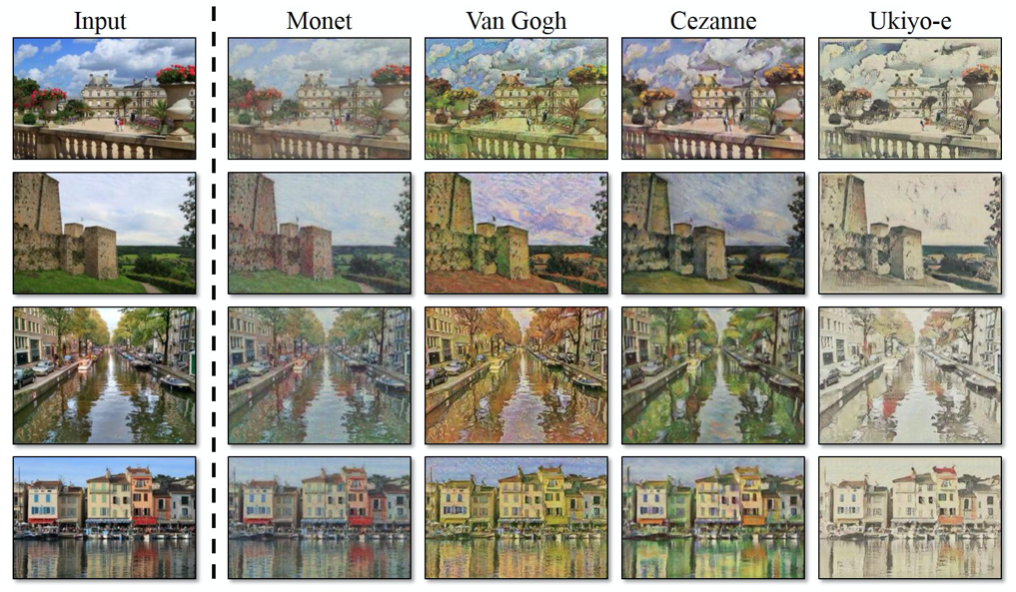
\includegraphics[width=0.45\textwidth]{resources/png/cyclegan-example.png}
        \caption{An example of neural style transfer produced by CycleGAN \cite{junyanz.github.io}.}
        \label{fig:introduction.example.cyclegan}
    \end{figure}
    
    We have also tried to re-implement it by ourselves and to vary its different elements. This method is described in section \ref{methods.zhu} and its results are discussed in section \ref{results.zhu}.\\
    
    Finally, we have tried some extensions in order to delve deeper into the subject : application of neural style transfer without going through a neural network (for comparison), extensions of the application such as controlling the color and adjust the style, etc.
    
    %%%%%%%%%%%%%%%%%%%%
    %%%%%%%%%%%%%%%%%%%%
    %%%%%%%%%%%%%%%%%%%%
    
    % ----- Related work ----- %
    
    % TO DO
    % -----
    % Research that is related to the considered problem
    
    \section{Related work}
    
    The field of neural style transfer and its applications are very rich. We have researched the literature to find out what the basic principles of this technique are, what the different techniques are and how they can be improved.\\
    
    We first based ourselves, as explained in the introduction, on the paper by Gatys et al. and on the paper by Zhu et al. :
    
    \begin{itemize}
        \item \cite{DBLP:journals/corr/GatysEB15a} - Paper by Gatys et al. : a paper that introduces a technique for neural style transfer using a network, such as VGG19, already trained.
        \item \cite{DBLP:journals/corr/ZhuPIE17} - Paper by Zhu et al. : a paper that introduces a technique, called CycleGAN, to perform unpaired image-to-image translation.
    \end{itemize}
    
    We then found a series of papers highlighting different discussions and improvement techniques :
    
    \begin{itemize}
        \item \cite{DBLP:journals/corr/GatysEBHS16} - Paper by Gatys et al. : a paper that follows their original one (\cite{DBLP:journals/corr/GatysEB15a}) and introduces several improvements concerning the results that can be obtained. Examples are the possibility to include bitmaps, to control the colour transfer and the scale.
    \end{itemize}
    
    %%%%%%%%%%%%%%%%%%%%
    %%%%%%%%%%%%%%%%%%%%
    %%%%%%%%%%%%%%%%%%%%
    
    % ----- Methods ----- %
    
    % TO DO
    % -----
    % A clear and detailed description of the neural networks (architecture, training-parameters, loss function, data)
    
    \section{Methods}
    
    \subsection{Neural style transfer (Gatys et al.)}\label{methods.gatys}
    
    The method presented in this section is that of the original paper that introduced neural style transfer. Although style transfer previously existed in a field called \emph{non-photorealistic rendering} and were implemented through \emph{artistic rendering} algorithms \cite{DBLP:journals/corr/JingYFYS17}, they made no use of neural networks for the task and achieved limited performance and results.\\
    
    The paper \cite{DBLP:journals/corr/GatysEB15a} makes use of convolutional neural networks to tackle the task. Those networks are the most powerful when dealing with images since they are able to quickly and efficiently detect local and global correlations in an image. Thanks to filters implemented at each layer, features of the image can be gradually extracted in a feedforward manner, from \textbf{smaller to greater details the more we advance or the contrary ?}. The outputs of each layer consist therefore in \emph{feature maps}, which are filtered versions of the input image.\\
    
    The authors decided to use networks that were pre-trained on object recognition tasks. Such a network creates a representation of the input image that makes the object information increasingly explicit during the treatment, and the content of the image is thus given more weight than the fine details. Higher-level layers contain high-level content while lower-level ones contain low-level details. High-level layers are thus used for content representation. On the other hand, the style is captured through correlations between the filter responses of different layers.\\
    
    The realization that made neural style transfer possible for the authors is that the style and content of an image are separable in a \emph{convolutional neural network}.\\
    
    As for the practical method proposed by the paper, they used the pretrained VGG19 network, consisting of 16 convolutional layers and 5 pooling ones (\textbf{explain somewhere what those are}). The responses in a layer $l$ being the features maps of that layer, they can be stored in a matrix $F^l \in \mathcal{R}^{N_l\times M_l}$, where $F_{ij}^l$ is the activation of the $i^{th}$ filter at position $j$ in layer $l$. $N_l$ is the number of distinct filters at layer $l$ and $M_l$ is the size of the feature map (height times width).\\ 
    
    The loss that the authors have used in their work is the following one :
    \begin{equation}
        \mathcal{L}_{total}(p,a,x) = \alpha \mathcal{L}_{content}(p,x) + \beta \mathcal{L}_{style}(a,x)
    \end{equation}
    where $p$ is the photograph (content image), $x$ is the constructed one and $a$ is the artwork (style image). Parameters $\alpha$ and $\beta$ are simply weighting factors controlling the tradeoff between style and content. The content loss is the mean square error between the response matrix of the content image and that of the constructed image, while the style loss is defined as the weighted sum of the mean square errors between the Gram matrices for the generated image and the style one, taken over all layers considered for the style. The \emph{Gram matrix} is a mathematical element that computes the correlation between the different filter responses for a given layer.
    
    \subsection{CycleGAN (Zhu et al.)}\label{methods.zhu}
    
    CycleGAN is neural networks that allows to perform \emph{unpaired image-to-image translation}. As described on its official web page, "\emph{image-to-image translation is a class of vision and graphics problems where the goal is to learn the mapping between an input image and an output image using a training set of aligned image pairs.}" \cite{junyanz.github.io}. However, in many cases, paired images are not available. This technique has therefore been designed to support unpaired images.\\
    
    Paired images are images with a common context and common elements (for example, an image of horse in a field and an image of a zebra in the same position in more or less an identical field) while unpaired images are images that are not really the same (for example, an image of a horse in a field and an image of a zebra, not in the same position, not in the same size and not in a field).\\
    
    CycleGAN uses a \emph{generative adversarial network}.
    
    \subsubsection{Generative models}
    
    \emph{Generative models} are models capable of learning how to create data similar to the data they are provided with (training data). Intuitively, a model acting on data (e.g. writing good scientific articles) must have a good internal representation of this data. This internal representation could then be exploited to perform other tasks (e.g. classifying scientific articles).\\
    
    More practically, a generative model is a model that attempts to learn the joint probability distribution $P(x,y)$ between data $x$ and their label $y$ (where a non-generative model learns the conditional probability $P(y|x)$). Thus, the model would be able to generate a new sample $(x,y)$.
    
    \subsubsection{Generative adversarial networks}
    
    \emph{Generative adversarial networks} are models whose main idea is to put in competition two neural network models. One is called the \emph{generator} and is in charge of generating noisy data. The other is called the \emph{discriminator} and receives the training data and the noisy data from the generator and has to be able to distinguish between the two sources.\\
    
    An illustration of the structure of a generative adversarial networks is presented in Figure \ref{fig:methods.cyclegan.gan}.
    
    \begin{figure}[ht]
        \centering
        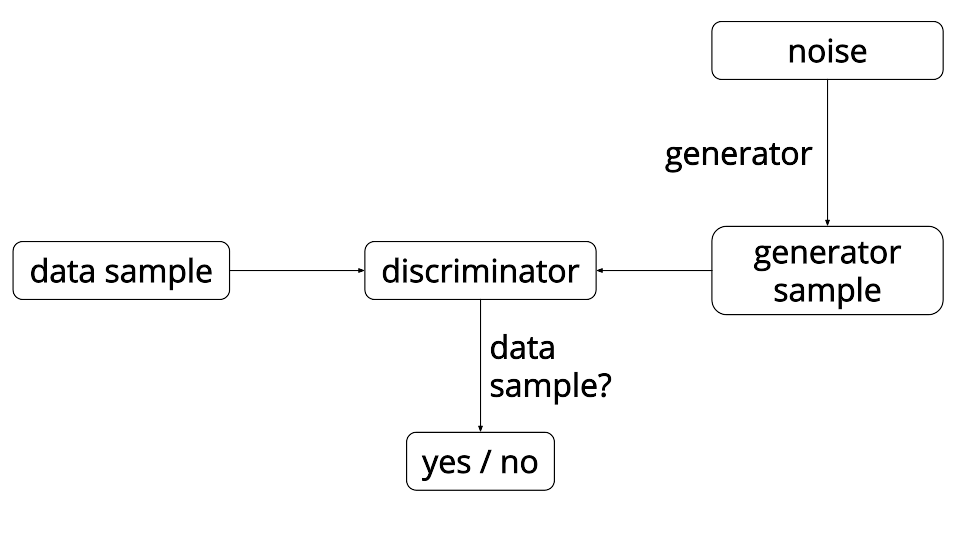
\includegraphics[width=0.45\textwidth]{resources/png/gan.png}
        \caption{Generative adversarial networks structure \cite{blog.aylien.com}.}
        \label{fig:methods.cyclegan.gan}
    \end{figure}
    
    As the training progresses, the generator produces less and less noisy data and the discriminator becomes better at distinguishing the source from the data it receives. The ultimate goal is to make the generator generate data that will be indistinguishable from the training data by the discriminator.\\
    
    In such a model, we can backpropagate gradient information from the discriminator back to the generator network, so the generator knows how to adapt its parameters in order to produce output data that can fool the discriminator.
    
    \subsubsection{CycleGAN}
    
    Coming back to the application of neural style transfer, the idea behind the use of a generative adversarial network is \emph{to learn a mapping between the input image and the output image}. However, this technique works for paired images. CycleGAN is a technique that works on unpaired images (or more generally, unpaired input data). For example, it will be able to transform a horse in a photo into a zebra (by applying a striped texture to it) without even needing a zebra image in the same position, with the same background, etc. (i.e. paired images of horse and zebra).\\
    
    The operating principle of CycleGAN is as follows : let one set of images (for example, images of horses) in an $X$ domain and another different set of images (for example, images of zebras) in a $Y$ domain. The goal is to obtain, via training, a mapping $G : X \rightarrow Y$ and a mapping $F : Y \rightarrow X$. Mathematically, $G$ and $F$ should be inverse to each other and both mapping should be bijections. This hypothesis being made, $G$ and $F$ are trained simultaneously via a \emph{cycle consistency loss} that encourages $F(G(x)) = x$ and $G(F(y)) = y$.\\
    
    The creators of CycleGAN have in fact exploited the fact that a translation must be "\emph{cycle consistent}" using this technique. Concretely, this means, for example, that if a sentence is translated from English into French, the re-translation of the freshly obtained French sentence into English should give the original sentence.\\
    
    Exploiting this property avoids problems such as \emph{mode collapse} : the model could generate an image which is in the domain of $Y$, and which would therefore be validated by the discriminator, without having any link with the domain $X$ (for example, generating an image of a zebra that is always abd always the same and does not look anything like the image of the original horse).\\
    
    In total, the model contains two loss functions : an \emph{adversarial loss function} (since it is a generative adversarial model) and a \emph{cycle consistent loss function} (to take into account the cycle consistent property).\\
    
    The adversarial loss function is defined as
    \begin{align}
        \mathcal{L}_{\mathrm{GAN}}\left(G, D_{Y}, X, Y\right)&=\mathbb{E}_{y \sim p_{\text {data }}(y)}\left[\log D_{Y}(y)\right]\nonumber\\
        &+\mathbb{E}_{x \sim p_{\text {data }}(x)}\left[\log \left(1-D_{Y}(G(x))\right]\right.
    \end{align}
    where $D_Y$ is a discriminant which aims to distinguish the images ${y}$ from the translated images ${G(x)}$. They also consider the same loss for $D_X$.\\
    
    The cycle consistent loss function is defined as
    \begin{align}
        \mathcal{L}_{\text {cyc }}(G, F) &=\mathbb{E}_{x \sim p_{\text {data }}(x)}\left[\|F(G(x))-x\|_{1}\right]\nonumber\\
        &+\mathbb{E}_{y \sim p_{\text {data }}(y)}\left[\|G(F(y))-y\|_{1}\right]
    \end{align}
    taking into account that the result must satisfy the \emph{forward cycle consistency} ($x\rightarrow G(x)\rightarrow F(G(x))\approx x$) and the \emph{backward cycle consistency} ($y\rightarrow F(y)\rightarrow G(F(y))\approx y$).\\
    
    An illustration of the cycle consistent loss is shown in Figure \ref{fig:methods.cyclegan.cycleconsistentloss}.\\
    
    \begin{figure}[ht]
        \centering
        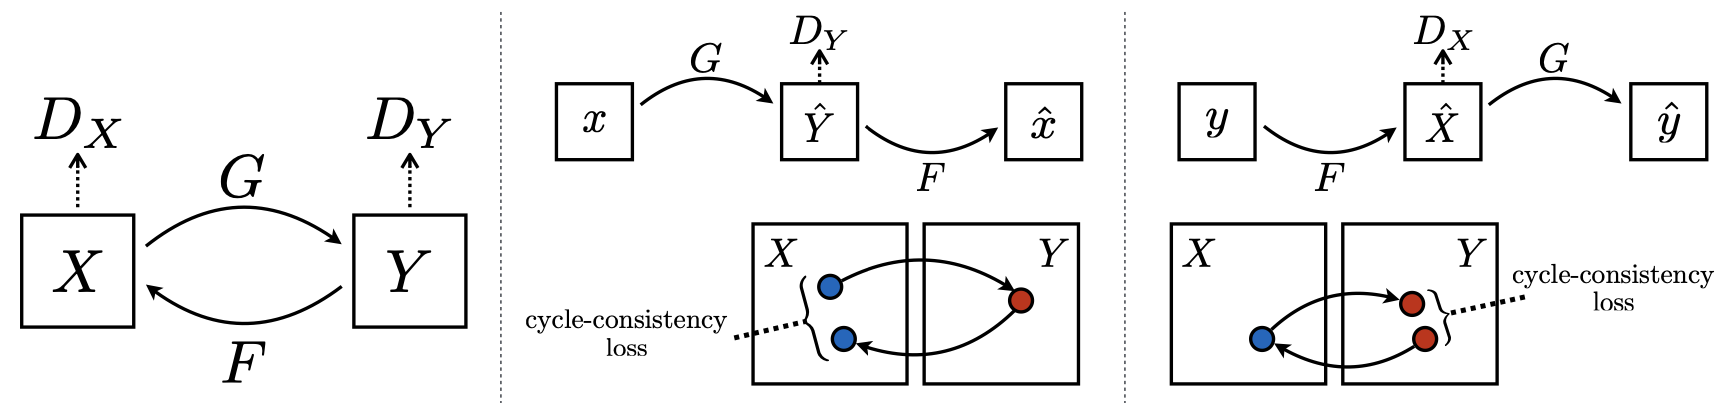
\includegraphics[width=0.45\textwidth]{resources/png/cycle-consistent-loss.png}
        \caption{Cycle consistent loss \cite{DBLP:journals/corr/ZhuPIE17}}
        \label{fig:methods.cyclegan.cycleconsistentloss}
    \end{figure}
    
    Finally, the total loss function that the model tries to minimize is defined as
    \begin{align}
        \mathcal{L}\left(G, F, D_{X}, D_{Y}\right) &=\mathcal{L}_{\mathrm{GAN}}\left(G, D_{Y}, X, Y\right)\nonumber\\
        &+\mathcal{L}_{\mathrm{GAN}}\left(F, D_{X}, Y, X\right) \\ &+\lambda \mathcal{L}_{\mathrm{cyc}}(G, F)
    \end{align}
    where $\lambda$ controls the relative importance of the two objectives.
    
    \subsubsection{Network architectures}
    
    Concerning generator architectures, authors of CycleGAN use architecture from Johnson et al. \cite{DBLP:journals/corr/JohnsonAL16} : 6 residual blocks for $128 \times 128$ training images and 9 residual blocks for $256 \times 256$ or higher-resolution training images.\\
    
    Concerning the discriminator architectures, they use a $70 \times 70$ PatchGAN.
    
    \subsubsection{Implementation}
    
    In order to implement the CycleGAN, we decided to not base ourselves upon a tutorial but instead to try to recreate the models and its training from the paper \cite{DBLP:journals/corr/ZhuPIE17} itself. The network architecture is referenced in the fourth section of this paper and makes reference to the network used in another paper \cite{DBLP:journals/corr/JohnsonAL16}. The exact architecture of the networks of this paper being given in the supplementary and using the discriminator architecture of \cite{DBLP:journals/corr/LedigTHCATTWS16}. We therefore tried to implement our network based on these sources and finished doing so before realizing that the exact architectures of CycleGan were given in the appendix of their paper, located after the sources. We thus used that source to modify the networks created to have the same basis as them. For the generator, we did not modify anything since the architecture we used and modified based on their comment in their own implementation was the same as the one provided in their appendix. For the discriminators, however, we had to modify our architecture since they did not mention that the kernel sizes were of 4, and so we went with the kernel size of 3 referenced by the original paper they based upon, and they used a stride of 2 for all layers, which was not the case in \cite{DBLP:journals/corr/LedigTHCATTWS16}. The number of blocks they used also differed.\\
    
    Finally, after having implemented the network, we went to their GitHub repository for the paper and compared our architecture and theirs, to make sure everything was correct. The only modification we had to make was change some reflection padding to simple padding with 0. They mentioned in their paper they used reflection padding to reduce artifacts but it was not done for all convolutional layers, so we modified that.\\
    
    After the network architectures, we had to acquire a dataset of images and paintings. To do so, we used a bash script found on their GitHub repository that downloads the same datasets as they used in their research. We decided to use landscapes and Monet paintings for the two domains of interest. We also had to create a custom data loader that would return an image of both domain when called, and to do so we looked into PyTorch documentation and StackOverflow questions.\\
    
    For the optimizer, we reused the same as the authors, and created a learning rate scheduler based on what they wrote in their paper.
    
    %%%%%%%%%%%%%%%%%%%%
    %%%%%%%%%%%%%%%%%%%%
    %%%%%%%%%%%%%%%%%%%%
    
    % ----- Results ----- %
    
    % TO DO
    % -----
    % Qualitative analysis : could include examples of generated images, correct vs wrong predictions, ...
    % Quantitative analysis : general overview of final performance, loss curves, comparison table with error-bars, ...
    
    \section{Results}
    
    \subsection{Neural style transfer (Gatys et al.)}\label{results.gatys}
    
    to do
    
    \subsection{CycleGAN (Zhu et al.)}\label{results.zhu}
    
    to do
    
    %%%%%%%%%%%%%%%%%%%%
    %%%%%%%%%%%%%%%%%%%%
    %%%%%%%%%%%%%%%%%%%%
    
    % ----- Discussion ----- %
    
    % TO DO
    % -----
    % A critical discussion of the performance of the neural network, analysis of the potential limitations, tips for future work
    
    \section{Discussion}
    
    to do
    
    %%%%%%%%%%%%%%%%%%%%
    %%%%%%%%%%%%%%%%%%%%
    %%%%%%%%%%%%%%%%%%%%
    
    % ----- References ----- %
    
    \bibliographystyle{unsrt}
    \bibliography{references.bib}
    \nocite{*}
\end{document}
